\documentclass[10pt,pdf,hyperref={unicode}]{beamer}

% \documentclass[aspectratio=43]{beamer}
% \documentclass[aspectratio=1610]{beamer}
% \documentclass[aspectratio=169]{beamer}

\usepackage{lmodern}

% подключаем кириллицу 
\usepackage[T2A]{fontenc}
\usepackage[utf8]{inputenc}

\usepackage{amssymb,amsfonts,amsmath,mathtext,cite,enumerate,amsthm,mathenv} %подключаем нужные пакеты расширений

% отключить клавиши навигации
\setbeamertemplate{navigation symbols}{}

% тема оформления
\usetheme{CambridgeUS}

\makeatother
\setbeamertemplate{footline}
{
  \leavevmode%
  \hbox{%
  \begin{beamercolorbox}[wd=.12\paperwidth,ht=2.25ex,dp=1ex,center]{author in head/foot}%
    \usebeamerfont{author in head/foot}\insertshortauthor
  \end{beamercolorbox}%
  \begin{beamercolorbox}[wd=.88\paperwidth,ht=2.25ex,dp=1ex,center]{title in head/foot}%
    \usebeamerfont{title in head/foot}\insertshorttitle\hspace*{1em}
    \insertframenumber{} / \inserttotalframenumber\hspace*{1ex}
  \end{beamercolorbox}}%
  \vskip0pt%
}
% цветовая схема
\usecolortheme{seahorse}

\graphicspath{{images/}}%путь к рисункам

\title[Удаление космического мусора путем электростатического взаимодействия с активным КА]{Выпускная квалификационная работа магистра\\
Удаление космического мусора путем электростатического взаимодействия с активным космическим аппаратом}
\author[Асланов Е.В.]{Научный руководитель: д.т.н., проф. Асланов В. С.\\
Выпускник: Асланов Е.В. гр. 1225 М 403}
\date[]{}
% \logo{\includegraphics[height=5mm]{images/logo.png}\vspace{-7pt}}

\begin{document}

% титульный слайд
\begin{frame}
	\titlepage
	\begin{center}
		Самара, 2017
	\end{center}
\end{frame} 

\begin{frame}
\frametitle{Цель и основные задачи работы}
		Цель – исследование применения метода многих сфер при моделировании движения относительно центра масс при электростатическом взаимодействии и рассмотрение управления для такой модели.
		
		Задачи:
		\begin{itemize}
				\item Моделирование движения космического аппарата цилиндрической формы вокруг центра масс с активным спутником при поддержании постоянного расстояния между центрами масс двух космических аппаратов методом многих сфер,
				\item Моделирование движения двух космических аппаратов как двух материальных точек при действии тяги на одном из них,
				\item Моделирование движения пассивного космического аппарата цилиндрической формы и активного космического аппарата методом многих сфер.
		\end{itemize}
\end{frame}

\begin{frame}
\frametitle{Метод  многих сфер}
\framesubtitle{Концептуальное описание метода многих сфер}
	\begin{figure}[H]
		\center{\includegraphics[scale=0.2]{spacecraft_msm.png}}
	\end{figure}
	\footnotesize{\textit{Daan Stevenson and Hanspeter Schaub. Multi-sphere method for modeling electrostatic forces and torques: Advances in Space Research, 51(1):10–20, Jan. 2013.}}
\end{frame}

\begin{frame}
\frametitle{Метод  многих сфер}
\framesubtitle{Вычисление зарядов}
	\begin{equation*}
		\vec{\Phi} = k_c [C_m]^{-1} \vec{q},
	\end{equation*}
	\footnotesize{где $k_c = \frac{1}{4\pi\varepsilon_0} = 8.99 * 10^9 \frac{N*m^2}{C^2}$ – постоянная Кулона, $\vec{\Phi} = [\Phi_A, \Phi_A, \dots, \Phi_A, \Phi_B]^T$ – вектор напряжений, $\vec{q} = [q_1, q_2, \dots, q_n, q_b]^T$ – вектор зарядов, $\Phi_A$ – напряжение каждой сферы тела, $\Phi_B$ – напряжение внешней сферы, $q_i$ – заряд $i$-ой сферы, $C_m$ – матрица ёмкостей.}
	
	\begin{equation*}
		[C_m]^{-1} = 
		\begin{pmatrix}
			1/R_1	&	1/r_{1,2}	&	\dots		&	1/r_{1,n}	&	1/r_{1,B} \\
			1/r_{1,2}	&	1/R_1	&	\dots		&	\vdots		&	\vdots \\
			\vdots		&	\ddots		&	\ddots	&	\vdots		&	\vdots \\
			1/r_{n,1}	&	\dots			&	\dots		&	1/R_n	&	1/r_{n,B} \\
			1/r_{B,1}	&	\dots			&	\dots		&	1/r_{B,n}	&	1/R_B
		\end{pmatrix},
	\end{equation*}
	\footnotesize{где $\vec{r}_{i,B} = \vec{d} - \vec{r}_i$.}
\end{frame}

\begin{frame}
\frametitle{Моделирование движения КА вокруг центра масс с помощью метода многих сфер}
\framesubtitle{Замена КА набором сфер}
	\begin{figure}[H]
		\center{\includegraphics[scale=0.3]{3sph.png}}
	\end{figure}
\end{frame}

\begin{frame}
\frametitle{Моделирование движения КА вокруг центра масс с помощью метода многих сфер}
\framesubtitle{Уравнения движения}
\begin{columns}[onlytextwidth]
	\begin{column}{0.5\textwidth}
	\begin{equation*}
		[C_m]^{-1} = 
		\begin{pmatrix}
			1/R_1	&	1/r_a	&	1/r_b	&	1/r_c\\
			1/r_a	&	1/R_{2a}	&	1/l		&	1/2l\\
			1/r_b	&	1/l		&	1/R_{2b}	&	1/l\\
			1/r_c	&	1/2l		&	1/l		&	1/R_{2c}
		\end{pmatrix},
	\end{equation*}	
	\begin{equation*}
		T = \frac{J \left(\frac{d \theta (t)}{dt}\right)^2}{2},
	\end{equation*}
	\begin{equation*}
		Q_\theta = \frac{\partial \vec{r}_{ba}}{\partial \theta(t)} \cdot F_{2a} + \frac{\partial \vec{r}_{bc}}{\partial \theta(t)} \cdot F_{2c},
	\end{equation*}
	\end{column}
	\begin{column}{0.5\textwidth}
	\begin{equation*}
		\begin{pmatrix}
			q_1\\
			q_{2a}\\
			q_{2b}\\
			q_{2c}
		\end{pmatrix}
		= k_c C_m 
		\begin{pmatrix}
			-\phi\\
			\phi\\
			\phi\\
			\phi
		\end{pmatrix},
	\end{equation*}
	\begin{equation*}
		F_{2a} = - \frac{k_c q_1 q_{2a}}{r_a^3}  R_a,
	\end{equation*}
	\begin{equation*}
		F_{2c} = - \frac{k_c q_1 q_{2c}}{r_c^3} R_c,
	\end{equation*}
	\end{column}
\end{columns}
\begin{center}
$S_a = - k_c q_1 q_{2a}$ и $S_c = - k_c q_1 q_{2c}$.
\end{center}
\end{frame}

\begin{frame}
	\begin{center}
		Спасибо за внимание!
	\end{center}
\end{frame}
\end{document}